\section{Alternative Method - kNN Regressor}
\label{sec:Alternative Method}

As an alternative approach, a simple kNN regressor of sklearn is utilized, as the true pricing is expected to be
highly influenced by similar motorcycles, such as motorcycles within the same brand or similar power. For the kNN classifier,
the same Pipeline as for the evaluation of the other models is employed. The regressor is trained for the different
scaling methods introduced in \autoref{sec:regression_models}, optimised with a RandomizedSearchCV grid search and 
evaluated with the same metrics as the other models.\\
The metrics of the best-performing kNN regressor are listed in \autoref{tab:kNN_metrics}. The kNN regressor
appears to perform slightly worse in every computed metric, except the training time. Considering the remarkably low
training time, an extensive hyperparameter optimisation or an application on a bigger dataset might be applicable.
\begin{table}[h!]
    \centering
    \begin{tabular}{ |p{3cm}||p{2cm}||p{2cm}|p{2cm}|p{2cm}|p{1.2cm}|  }
        \hline
        \multicolumn{6}{|c|}{Evaluation kNN Regressor} \\
        \hline
        RMSE / €  & MSE / €  & MAE / € & $ \mathrm{R}^2 $ Test& $ \mathrm{R}^2 $ Train & TT / s \\
        \hline
        $2515.53 \pm  415.84$ & $ 5167510.12$ & $1418.12$ & $0.877$ & $0.995$ & $0.02$\\
        \hline
      \end{tabular}
      \caption{RMSE, MSE, MAE, $R^2$ score for training and testing and training time for the kNN regressor.}
      \label{tab:kNN_metrics}
\end{table}

\subsection{Comparison to Ensembled Model}

The comparison of the computed quality measures for the ensembled model and the kNN regressor indicates a better
overall performance of the ensembled model. However, the achieved performance of the 
kNN regressor is still better than for some of the other individually trained models, which makes the kNN
model a potential candidate to achieve a higher overall performance in the ensembled regressor.\\
Taking the difference of $ \mathrm{R}^2 $ score of the training and testing dataset, there
are significant indications of potential overtraining. This issue can 
be addressed by the implementation of regularisation techniques and a more aggressive feature selection process involving the removal of many 
attributes with low feature importance.\\
As demonstrated by the residuals in the scatter plot in \autoref{fig:res_knn_ens}, both regressors seem to 
overestimate the price in lower ranges and underestimate it for higher values. This observation aligns with the already mentioned concern
of many outliers, as special editions or very bad conditions cannot be predicted
by the regressor model. The projected histogram of the residuals on the right shows, that the kNN regressor seems
to have a higher spread in general and a higher tendency towards underestimating the price. 
\begin{figure}
\centering
    \makebox[\textwidth][c]{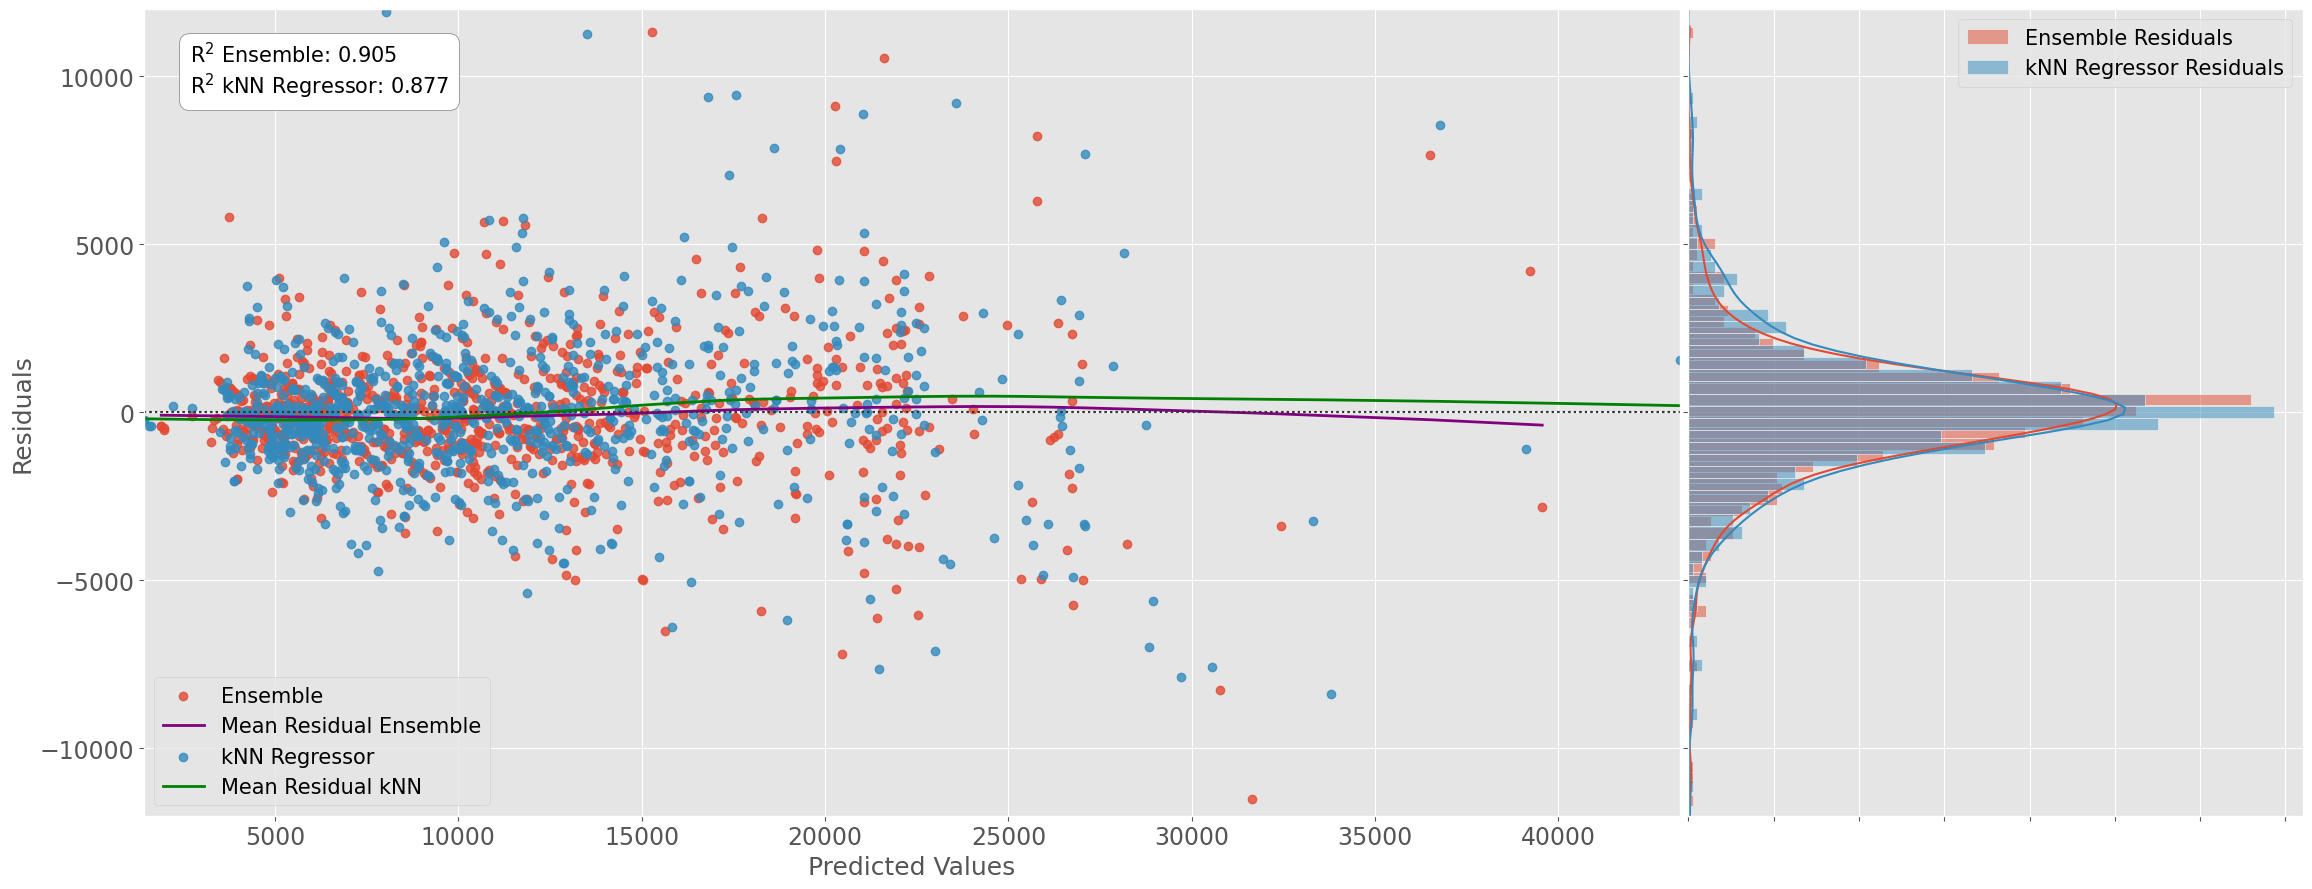
\includegraphics[width=1\textwidth]{"content/pics/residuals_Ensemble_kNN.png"}}
    \caption{Residuals for different predicted prices for the ensembled model for training and testing subsets.}
    \label{fig:res_knn_ens}
\end{figure}
\\ Although the ensembled model performs better than the alternative approach of a kNN regressor, the CatBoost regressor performs
almost equally well. Hence, there is no justification to use an ensembled model over the individual CatBoost regressor. The CatBoost
regressor might perform best in this dataset, as many attributes selected as important by the feature selection, seem to have a categorical
origin.\\
Further plots comparing the performance of the ensembled model with the kNN regressor are not included in this chapter due to a lack of space and 
are included in the \autoref{sec:Appendix}.
    
\newpage